\documentclass{article}
\usepackage{geometry}
\geometry{
	a4paper,
	total={170mm,257mm},
	left=20mm,
	top=20mm,
}
\usepackage{amsmath}
\usepackage{amssymb}
\usepackage{graphicx}
\graphicspath{ {./images/} }
\usepackage[utf8]{inputenc}
\usepackage{epigraph}
\title{Multi-Period Asset Pricing}
\date{Nov 16th 2018}
\author{Xia Xicheng}

\begin{document}
	\maketitle

\section{Hansen–Jagannathan Bound}
\begin{figure}[h]
	\centering
	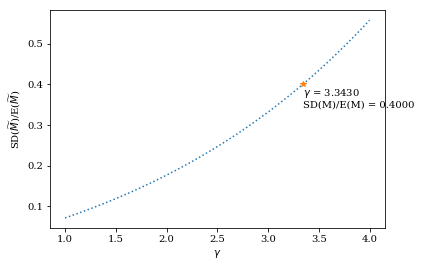
\includegraphics[width=9cm]{output_4_0.png}
\end{figure}

\begin{itemize}
	\item The ratio of the standard deviation of a stochastic discount factor ($\tilde{M}$) to its mean exceeds the Sharpe Ratio attained by anyportfolio.
	
	\item The higher the $\gamma$ is, the more the investor risk averse, the lower variance they require for the same asset return.
	
	\item For those who have a risk averse level of 3.3430, the sharpe ratio requiremnet for they investment is 0.4 
\end{itemize}

\section{Price-Dividend Ratio}
\begin{figure}[h]
	\centering
	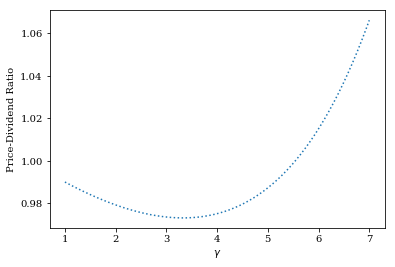
\includegraphics[width=9cm]{output_6_0.png}
\end{figure}
\newpage
\section{Equity Premium}
\begin{figure}[h]
	\centering
	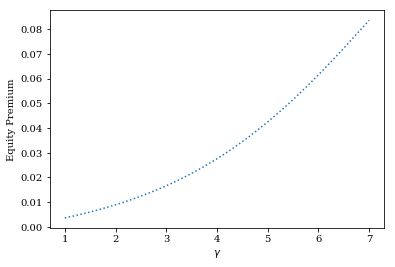
\includegraphics[width=9cm]{output_7_0.png}
\end{figure}
\end{document}